% !TeX root = CoPhy-Projekt.tex

%----------------------------------------------------------------%
%--------------------------GRUNDEINSTELLUNGEN--------------------%
%----------------------------------------------------------------%
\documentclass[oneside, ngerman, footinclude=off, captions=tableheading]{scrartcl}
%	'oneside'/'twoside': nicht zwischen linker und rechter Seite unterscheiden (alternativ twoside)
%	'twocolumn': wuerde 2 Spalten auf dem Blatt platzieren
%	'bibliography=totocnumbered': Normal nummeriertes Inhaltsverzeichnis (Kapitelnummer)
%	'listof=totocnumbered': Abbildungs- und Tabellenverzeichnis normal nummeriert (Kapitelnummer)
%	'ngerman' verwendet deutsch als Dokumentensprache (z.B. fuer Sirange)
%	'footinclude=off': Zaehlt Fusszeile zum Rand (vergroessert den Textbereich)
%	'captions=tableheading': Tabellenueberschriften explizit verwenden, erhoeht den Abstand zur Tabelle

\usepackage[ngerman]{babel}		%	Einstellen der Sprache
\usepackage[T1]{fontenc}		%	Wie wird Text ausgegeben, d.h. im PDF
\usepackage[utf8]{inputenc}		%	Welche Zeichen 'versteht' LaTeX bei der Eingabe?
\usepackage{lmodern}			%	Laedt Schriften, die geglaettet sind
\usepackage{blindtext}			%	Beispieltext, zum Testen geeignet

%----------------------------------------------------------------%
%--------------------------ABSTÄNDE------------------------------%
%----------------------------------------------------------------%
%\usepackage[onehalfspacing]{setspace}				%	Für Zeilenabstaende: 'singlespacing' (einfach), 'onehalfspacing' (1.5-fach), 'doublespacing' (2fach)
%\setlength{\parindent}{0cm}						%	Laengenangabe für die Einrueckung der ersten Zeile eines neuen Absatzes.
%\setlength{\parskip}{6pt plus 3pt minus 3pt}		%	Laengenangabe für den Abstand zwischen zwei Absaetzen.
%	Wenn diese beiden Befehle nicht kommentiert sind, wird ein Absatz nicht eingezogen sondern es gibt einen Abstand

% kleinere Abstände über und unter Gleichungen
\usepackage{setspace}\onehalfspacing
\AtBeginDocument{%
  \addtolength\abovedisplayskip{-0.2\baselineskip}
  \addtolength\belowdisplayskip{-0.2\baselineskip}
}

%----------------------------------------------------------------%
%--------------------------MATHE---------------------------------%
%----------------------------------------------------------------%
\usepackage[]{mathtools}							%	Erweiterung von AMSMath, laedt automatisch AMSMath - für viele Mathe-Werkzeuge, 'fleqn' als Option ist für Mathe linksbuendig
\usepackage{amsfonts}								%	Für eine Vielzahl an mathematischen Symbolen
\usepackage{nicefrac}

%----------------------------------------------------------------%
%--------------------------KOPF- UND FUSSZEILEN------------------%
%----------------------------------------------------------------%
\usepackage[automark,headsepline=.4pt]{scrlayer-scrpage}
\pagestyle{scrheadings}
\setkomafont{pageheadfoot}{\normalfont\bfseries}	%	Normale Schriftart und Fett für den Seitenkopf
\addtokomafont{pagenumber}{\normalfont\bfseries}	%	Normale Schriftart und Fett für die Seitenzahl
\clearpairofpagestyles								%	Löscht die Seitenkopf- und Seitenzahlen
\ohead{\thepage}									%	Rechter Seitenkopf mit Seitenzahl
\ihead{\headmark}									%	Linker Seitenkopf mit section
\ofoot[]{\empty}									%	Leere Fußzeile, ungerade Seiten
%	Definert man oben in der documentclass 'twoside', so wird zwischen geraden und ungeraden Seiten unterschieden (NUR DANN!)

%----------------------------------------------------------------%
%--------------------------BILDER--------------------------------%
%----------------------------------------------------------------%
\usepackage{graphicx}									%	Um Bilder einbinden zu koennen 
\usepackage[dvipsnames,svgnames,table]{xcolor}			%	Farben verwenden, Versch. Farbdefinitionen, Farben in Tabellen (-Reihen, -Spalten)
\usepackage{pdfpages}									%	pdfs importieren
\definecolor{Seeblau100}{RGB}{0,169,224}				%	Uni-Farben, z.B. fuer Tabellen
\definecolor{Seeblau65}{RGB}{89,199,254}
\definecolor{Seeblau35}{RGB}{165,224,254}
\definecolor{Seeblau20}{RGB}{203,237,254}
\definecolor{Seegrau60}{RGB}{102,102,102}
\definecolor{Seegrau40}{RGB}{153,153,153}
\definecolor{Seegrau20}{RGB}{204,204,204}
\definecolor{Seegrau10}{RGB}{230,230,230}

%----------------------------------------------------------------%
%--------------------------POSITIONIERUNG------------------------%
%----------------------------------------------------------------%
\usepackage{float}

%----------------------------------------------------------------%
%--------------------------LISTEN--------------------------------%
%----------------------------------------------------------------%
\usepackage{enumitem}							%	Um Listen / Aufzaehlungen leichter zu modifizieren
%\setlist{noitemsep}							%	Verringert den Abstand in Aufzaehlungen

%----------------------------------------------------------------%
%--------TABELLEN-/BILDUNTERSCHRIFTEN und NUMMERIERUNG-----------%
%----------------------------------------------------------------%
\addtokomafont{captionlabel}{\bfseries}			%	Abbildung X.Y wir fett geschrieben
\setcapindent{2em}								%	2. Zeile teilweise haengend und eingezogen. Wenn ganz haengend gewuenscht, auskommentieren


%----------------------------------------------------------------%
%--------------------------LITERATURVERZEICHNIS------------------%
%----------------------------------------------------------------%
\usepackage[german]{babelbib}					%	Bereitstellung des deutschen Layouts fuer die Bibliography
\bibliographystyle{babalpha}

%----------------------------------------------------------------%
%--------------------------SIUNITX-------------------------------%
%----------------------------------------------------------------%
\usepackage[]{siunitx}
\DeclareSIUnit\octave{oct}
\DeclareSIUnit\Hz{Hz}
\sisetup{locale = DE}							%	Automatische Einstellung der Ausgabe für bestimmte Regionen (UK, US, DE, FR, ZA)
\sisetup{separate-uncertainty = false
}

%----------------------------------------------------------------%
%--------------------------URLs / REFs---------------------------%
%----------------------------------------------------------------%
\usepackage[hidelinks]{hyperref}				%	Erweiterte Referenzierung ('hidelinks' verhindert Linien um Links)

%----------------------------------------------------------------%
%--------------------------EIGENE BEFEHLE------------------------%
%----------------------------------------------------------------%

\usepackage{todonotes}
\usepackage{wrapfig}
\setlength{\intextsep}{0pt}%
\usepackage{multicol}

\usepackage{listings}
\usepackage{xcolor}

\definecolor{codegreen}{rgb}{0,0.6,0}
\definecolor{codegray}{rgb}{0.5,0.5,0.5}
\definecolor{codepurple}{rgb}{0.58,0,0.82}
\definecolor{backcolour}{rgb}{0.95,0.95,0.92}

\lstdefinestyle{mystyle}{  
    commentstyle=\color{codegreen},
    keywordstyle=\color{magenta},
    numberstyle=\tiny\color{codegray},
    stringstyle=\color{codepurple},
    basicstyle=\ttfamily\footnotesize,
    breakatwhitespace=false,         
    breaklines=true,                 
    captionpos=t,                    
    keepspaces=true,                 
    numbers=left,                    
    numbersep=5pt,                  
    showspaces=false,                
    showstringspaces=false,
    showtabs=false,                  
    tabsize=2
}


\lstset{style=mystyle}


\begin{document}

\title{Computerphysik I: Swing-by Manöver}
\author{Aurel Müller-Schoenau, Leon Oleschko und Moritz Schröer}
\maketitle

\begin{abstract}	
\end{abstract}

\section{Einleitung}
Beim Swing-By geht es darum, einen Satelliten gezielt an einem Himmelsobjekt vorbeifliegen zu lassen, damit die wirkende Gravitation den Satelliten auf einen gewünschten Orbit bringt. Dadurch lässt sich der sonst zur Beschleunigung benötigte Treibstoff sparen.\\
In diesem Bericht geht es um eine historische Raumfahrtmission der ESA, es handelt sich um die Ulysses-Raumfahrtmission. Bei dieser wurde nur ein Swing-by, nämlich am Planeten Jupiter, durchgeführt und die Daten zur Flugbahn sind verfügbar\footnote{\url{https://www.cosmos.esa.int/web/ulysses/mission-trajectory}}. Ziel ist es, mithilfe einer Simulation anhand der Shooting-Methode herauszufinden, wie der Satellit von der Erde aus ins All geschickt werden muss, um einen Swing-By auf den entsprechenden Orbit zu erreichen, und dann den errechneten Orbit mit den historischen Daten zu vergleichen.

\section{Trajektorie}
\begin{figure}[h!]
	\centering
	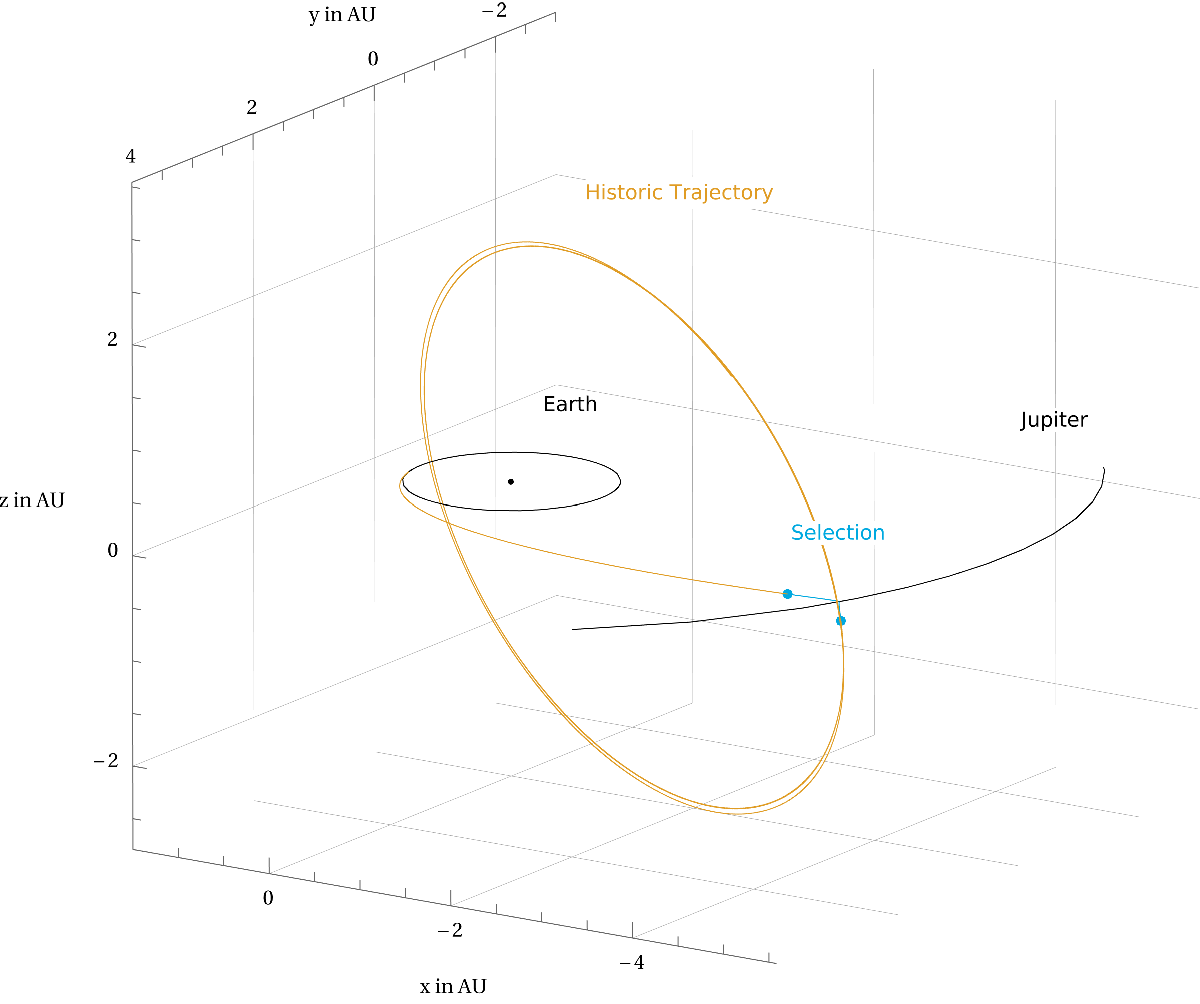
\includegraphics{img/trajectory.pdf}
	\caption{Abbildung der historischen Trajektorie, der simulierten Flugbahn und der relevanten Himmelskörpern}
	\label{fig:trajectory}
\end{figure}

Um die Flugbahn zu simulieren, muss die wirkende Gravitationskraft berechnet werden.
Zu Vereinfachung werden nur die Sonne, die Erde und der Jupiter berücksichtigt, weil der Satellit an keinem anderen Planeten nahe vorbeiflog.
Die Planeten-Daten wurden aus Mathematica\footnote{Wolfram Research, Inc., Wolfram|Alpha Notebook Edition, Champaign, IL (2022).} in gebräuchlicher Auflösung exportiert, um die Datenmenge zu reduzieren.
Da die Koordinaten nur tageweise vorliegen, werden sie in der Simulation linear über den Tag interpoliert.
In Abbildung \ref{fig:trajectory} sind die Positionen der Planeten, die Historische Trajektorie und ein simulierte Flugbahn dargestellt.

Für die Simulation wurde eine Dauer von 2800 Tagen betrachtet, wobei der Satellit historisch ungefähr 474 Tage für den Transfer zum Jupiter benötigte, und in der restlichen Zeit etwa einen vollständigen Orbit nach dem Swing-By durchlief.
Jeder dieser Tage wurde in 1000 Zeitschritte aufgeteilt, da bei mehr Schritten sich die Ergebnisse nicht mehr verändert haben.
Für jeden dieser Schritte wurde ein Leap-Frog-Schritt durchgeführt, um die Position und Geschwindigkeit des Satelliten zu berechnen. Dabei wurden die Positionen der Himmelskörper als vom Satelliten unbeeinflusst angenommen.


\begin{figure}[h!]
	\centering
	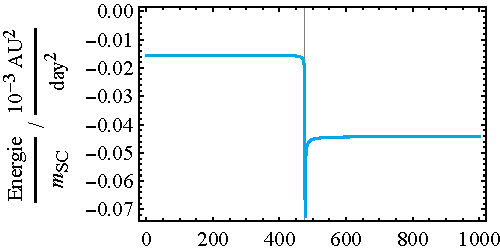
\includegraphics{img/energy.pdf}
	\caption{Energie und Geschwindigkeit während des Swing-by Manövers}
	\label{fig:energie}
\end{figure}


\section{Fehlerfunktionen}
\begin{figure}[h!]
	\centering
	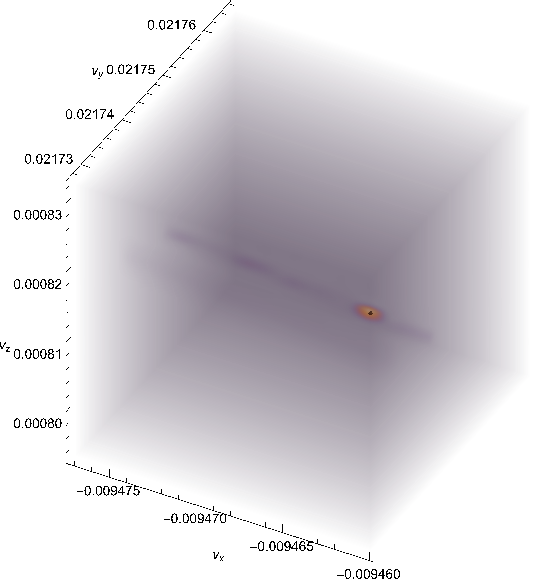
\includegraphics{img/gridSearch.pdf}
	\label{fig:gridSearch}
\end{figure}

Damit ein gewünschter Orbit erreicht werden kann, muss zunächst definiert werden, wie dieser aussehen soll. Der Starpunkt des Satelliten liegt natürlich auf der Erde. Den genauen Endzustand kennen wir im Fall der historischen Raumfahrtmission, ansonsten bleibt nur übrig, den gewünschten Zielorbit auf andere Weise zu definieren. In beiden Fällen handelt es sich um ein Randwertproblem, welches sich mithilfe der Shooting-Methode lösen lässt.\\
Dazu definieren wir eine Fehlerfunktion, die genau dann zu null wird, wenn der Satellit sich am Ende der Simulationszeit auf dem gewünschten Kurs befindet.
Um den Satelliten in unserer Simulation auf den finalen Orbit des Ulysses-Satelliten zu schicken, haben wir verschiedene Fehlerfunktionen ausprobiert.


\subsection{Vergleich der Endgeschwindigkeit und des Ortes}

Um einen Orbit zu erhalten, der dem historischen ähnelt, wurde zunächst \textit{zu einem festen Zeitpunkt} nach dem Swing-By der \textit{Ort und die Geschwindigkeit} des Satelliten mit den historischen Daten verglichen. Da diese keine Geschwindigkeitsinformationen enthalten, wurde dafür die mittlere Geschwindigkeit des Tages angenommen. \\
Der Ort allein als Vergleichswert reichte nicht aus, da das Programm sonst eine Abkürzungslösung fand, bei der der Satellit an der (im Vergleich zu den historischen Daten) entgegengesetzten Seite des Jupiter vorbeiflog, dadurch jedoch beim Swing-By in die falsche Richtung, und somit nicht auf den gewünschten Orbit abgelenkt wurde.

\subsection{Mehre Endpunkte zu festen Zeiten}

Eine andere Methode ist der Vergleich der \textit{Ort}skoordinaten nach dem Swing-By \textit{zu mehreren Zeitpunkten}, dafür aber \textit{ohne Vergleich der Geschwindigkeiten}. Der Zielorbit wird nun also durch eine Reihe an Wegpunkten definiert, die zu bestimmter Zeit zu erreichen sind.

\subsection{Integral des Ort-Fehler-Quadrates}

Bei dieser Fehlerfunktion wurde über ein Zeitintervall der Abstand zu den entsprechenden Wegpunkten des Zielorbits errechnet, und die Abstände wurden diesmal quadratisch aufaddiert. Als diskrete Annäherung des Integrals des Fehlerquadrats liefert dies eine Bewertung des Orbits, indem die Fläche zwischen errechnetem und Zielorbit betrachtet wird, das Quadrieren dient der stärkeren Gewichtung einzelner größerer Abweichungen gegenüber vieler leichter Abweichungen.


\subsection{Vergleich von Zielpunkten bei nächster Zeit}

Um die Tatsache, dass in der Realität bei der Planung eines Swing-By-Manövers wahrscheinlich keine passenden Daten vorlägen, nicht völlig außer Acht zu lassen, wurden bei der vierten Fehlerfunktion einige Punkte auf dem Wunsch-Orbit ausgewählt - in unserem Fall genau solche, die in den historischen Daten vorlagen, aber es hätten beliebige Punkte sein können. Und dann wurde beim Berechnen der Trajektorie bei jedem Zeitschritt der aktuelle Abstand zu jedem der ausgewählten Punkte gemessen. Der Wert wurde mit einem gespeicherten Wert verglichen, und dieser überschrieben, falls der aktuelle Wert kleiner war. So wurde zu jedem der ausgewählten Punkte der nächstgelegene Punkt der aktuellen Trajektorie gefunden.\\
Bei dieser Methode muss also der Zeitpunkt des Manövers nicht im Voraus bekannt sein, jedoch besteht die Möglichkeit, dass ein korrekter Orbit nicht erkannt wird, wenn die ausgewählten Punkte des gewünschten Orbits gerade zwischen denen des berechneten Orbits liegen. Solange die Zeitschritte klein genug sind, wird dann aber der Fehler immernoch sehr klein. Es wurde deshalb \textit{bei jedem Sub-Step}, also pro tausendstel Tag, der Abstand verglichen.






\section{Optimierung}
Die Shooting-Methode besteht nun darin, die Fehlerfunktion für einen gegebenen Orbit auszuwerten, und ausgehend davon den Orbit in irgendeiner Weise anzupassen, um schließlich die Nullstelle der Fehlerfunktion zu finden.
Als Optimierungsparameter wurde die Anfangsgeschwindigkeit gewählt, da diese nur 3 Dimensionen hat und somit leichter zu optimieren ist, als z.B. der Transferorbit.
Als initialer Wert wurde die echte gemessene Geschwindigkeit verwendet. Wichtig war vor allem, eine Anfangsgeschwindigkeit zu wählen, für welche der Satellit möglichst nahe am Jupiter vorbeifliegt, um die Laufzeit des Suchalgorithmus zu verringern. \\
Die historischen Daten liegen aber in Form von Kooridinaten in einem sphärischen heliozentrischen Koordinatensystem vor und haben eine Auflösung von $0.01\text{°}$.
Daraus lässt sich eine Unsicherheit der Position von $4\;\text{AU}\cdot\sin 0.01\text{°}\approx 7\cdot 10^{-4}\;\text{AU}$ und daraus eine Unsicherheit der Geschwindigkeit von $\sqrt{2}\cdot 7\cdot 10^{-4} \approx 10^{-3}\;\text{AU/day}$ abschätzen.
Solche Unsicherheit ist viel zu groß für die nötige Genauigkeit von $10^{-6}$ bis $10^{-8}\;\text{AU/day}$, denn so viele Stellen muss der Suchalgorithmus optimieren, um die Nullstelle der Fehlerfunktion möglichst genau zu finden. Eine sehr kleine Änderung der Startgeschwindigkeit kann bereits zu einem völlig anderen Orbit führen. Dies dämpft die Erwartungen an die Ergebnisse.\\
Zur Nullstellensuche wurden verschiedene Verfahren ausprobiert.

\subsection{Newton-Verfahren}

Die Nullstelle einer stetig differenzierbaren Funktion lässt sich mithilfe des Newton-Verfahrens finden. Dabei wird die Funktion lokal linear durch ihre Ableitung angenähert. Ist die Determinante der Ableitung ungleich Null, so lässt sich das entsprechende Gleichungssystem für jedes gewünschte Ergebnis eindeutig lösen. Die Nullstelle der Taylor-Entwicklung bis zur ersten Ordnung an einem beliebigen Startpunkt wird auf diese Weise bestimmt, und die Lösung wird als neuer Startwert für die nächste Iteration desselben Vorgehens verwendet. \\
Das Newton-Verfahren konvergiert unter bestimmten Bedingungen (die unsere Fehlerfunktionen erfüllen) lokal quadratisch gegen eine Nullstelle der untersuchten Funktion (ohne Beweis).

\subsection{Newton-Verfahren der Optimierung}

Um das Newton-Verfahren anwenden zu können, ist es also notwendig, dass die Fehlerfunktion genau so viele Ausgabewerte besitzt, wie es anzupassende Parameter gibt. Deshalb sind die Beschreibungen der Fehlerfunktionen immer Komponentenweise zu verstehen.\\
In der Optimierung gibt es ein gebäuchliches Verfahren, um \textit{lokale Extremstellen} einer Fehlerfunktion mit eindimensionalem Output zu finden. Dazu wird zunächst der Gradient berechnet, und darauf dann das Newton-Verfahren angewendet. Man rechnet also zunächst die Hesse-Matrix aus, und versucht dann wie im vorigen Abschnitt das Gleichungssystem zu lösen, um um sich iterativ einer Nullstelle zu nähern. \\
Wir haben im Rahmen dieses Projekts auch dieses Verfahren ausprobiert, indem es auf die quadratische Summe der Komponenten einer unserer Fehlerfunktionen angewendet wurde. Dann ist nämlich die Nullstelle der vorherigen Fehlerfunktion ein globales, und somit auch ein lokales Minimum der resultierenden Funktion. \\
Ein Problem dieses Verfahrens ist die lange Laufzeit, denn das numerische Berechnen der Hesse-Matrix läuft in quadratischer Zeit, im Gegensatz zur einfachen Ableitung, bei der der Aufwand nur linear ansteigt. Und da der Einfluss der Startparameter auf den End-Orbit des Satelliten untersucht wurde, musste hier für jeden Optimierungsschritt viel gerechnet werden, weshalb das Programm sehr lange lief, auch unter Verwendung der OMP-Library.


\subsection{Gradienten-Verfahren}

Ebenfalls zum finden lokaler Minima solcher Funktionen verwendet man das Gradienten-Verfahren. Dabei wird ebenfalls iterativ vorgegangen, jedoch bestehen die Iterationsschritte darin, dem Gradienten ein Stück weit zu folgen. Hier muss allerdings nur einmal abgeleitet werden, was die Rechenzeit wieder erträglich macht.

\vspace{1.5cm}

Es wurden verschiedene Verfahren verwendet, weil manchmal das eine, manchmal das andere Probleme mit der Konvergenz (bei gleichen Anfangsbedingungen) lieferte.

\section{Diskussion der Ergebnisse und Probleme}

\subsection{Was funktioniert hat}

Alle Optimierungsverfahren und alle hier beschriebenen Fehlerfunktionen lieferten plausible Ergebnisse, die gefundenen Startbedingungen führten in der Simulation tatsächlich zu Orbits, für welche der Satellit einen Swing-By durchführte. Weil eine kleine Positionsänderung \textit{zur Zeit des Swing-By}, also nach fast 500 Simulationszeit, zu einem komplett anderen End-Orbit führt, und nach letzterem optimiert wurde, sind alle gefundenen Orbits visuell vor dem Manöver nicht zu unterscheiden. In Abbildung \ref{fig:trajectory} ist nur ein simulierter Orbit dargestellt, es könnten aber auch alle sein. Sehen würde man es fast nicht, außer, dass die Trajektorien am Ende leicht auseinanderlaufen, aber auch hier kaum. Im Grunde funktionieren also die Simulation und auch die Optimierungsverfahren. In Abbildung \ref{fig:energie} ist schön zu sehen, wie sich beim Swing-By die Gesamtenergie von der des Startorbits zu der des Zielorbits ändert, und ansonsten zeitlich konstant bleibt.


\subsection{Was nicht funktioniert hat}

Bei den Berechnungen der Trajektorie konnten allerdings mit keiner der benutzen Methoden eine exakte Reproduktion der historischen Daten erreicht werden. Es gibt mehrere mögliche Fehlerquellen, die die Genauigkeit der Berechnungen einschränken. Eines der Probleme, welches alle bei diesem Projekt implementierten numerischen Optimierungsverfahren haben ist, dass diese nur lokal konvergent sind. Das entscheidende  Problem der lokalen Konvergenz kann dabei mittels der bei dem Projekt implementierten \glqq Grid-Search-Methode\grqq\, gezeigt werden. Bei der \glqq Grid-Search-Methode\grqq\, werden die Werte der verwendeten Fehlerfunktionen für ein feines Gitter von Anfangsgeschwindigkeiten berechnet. Das Gitter von Anfangsgeschwindigkeiten umfasst dabei einen gewissen Geschwindigkeitsbereich welcher sich um die gesuchte Anfagsgeschwindigkeit erstreckt. Dabei hat sich gezeigt, dass die untersuchten Fehlerfunktionen mehrere lokale Minima im Bereich der gesuchten Lösung besitzen, welche nur sehr geringe Abstände zueinander haben, nämlich teilweise in der Größenordnung $10^{-8}\;\text{AU/day}$ (vgl. Abbildung \ref{fig:gridSearch}). Das hat zur Folge, dass die lokal konvergenten Optimierungsverfahren nicht immer gegen die gesuchte Lösung konvergieren. Besonders beim Newton-Verfahren zur Suche von Minima (in Kapitel 4.2 beschrieben) hat sich gezeigt, dass dieses aufgrund der vielen lokalen Minima für diese Art von Problemstellung eher ungeeingnet ist.\\
Außerdem stellten wir nach einiger Zeit fest, dass die historischen Daten in unserer Simulation keinen möglichen Orbit darstellen. Wählt man als Anfangsgeschwindigkeit diejenige, die sich aus den echten Messwerten errechnen lässt, dann fliegt der Satellit so weit am Jupiter vorbei, dass gar kein Swing-By stattfindet. Der Vergleich eines gefundenen Orbits mit den historischen Daten zeigt, dass während des Flugs Kräfte gewirkt haben müssen, die wir nicht nachvollziehen können. Leider liegen uns keine Informationen dazu vor, ob, und wenn ja wann Triebwerke am Satelliten verwendet wurden, um den Orbit zu korrigieren. Diejenigen Orbits, die in unserer Simulation auf den gewünschten Zielorbit gelangen, erreichen den Jupiter immer etwa vier Tage zu spät (verglichen mit historischen Daten).

\subsection{Was man hätte besser machen können}

Von Anfang an wurde versucht, den historischen Orbit zu treffen, obwohl dieser keinen in unserer Simulation gültigen Orbit darstellte. Es ging viel Zeit dadurch verloren, die Probleme in den Fehlerfunktionen zu suchen, die dazu gedacht waren, den historischen Orbit zu finden, der ja gar nicht existierte (in unserem erfundenen Universum zumindest). Das alles hätte nicht passieren können, wenn man sich lediglich am Ziel-Orbit, und nie direkt an den Datenpunkten Orientiert hätte. Vor allem ist damit das Zeitproblem gemeint: Drei unserer vier Fehlerfunktionen verglichen Ort und eventuell Geschwindigkeit zu festen Zeitpunkten. Das Resultat waren Orbits, die mehrere Tage länger zum Jupiter brauchten, und dort dann etwas länger verweilten, um schließlich mit den (mit unserer Simulation nicht vereinbaren) historischen Daten \textit{zum richtigen Zeitpunkt} zusammenzutreffen. \\
Wir überlegten zwischenzeitlich, eine Ellipse auf die historischen Daten zu fitten, um eine Fehlerfunktion darüber zu definieren, das schien aber zu kompliziert. Schlauer gewesen wäre vielleicht eine Definition der Fehlerfunktion über die gewünschte Gesamtenergie, den gewünschten Drehimpulsbetrag bezüglich der Sonne, und den Abstand zur Ebene, in welcher der Orbit liegen sollte. Das hätte vielleicht bessere Ergebnisse geliefert, aber lässt sich im zeitlichen Rahmen nicht mehr überprüfen. 



\section{Fazit}

Es ist uns geglückt, anhand eines Optimierungsalgorithmus einen (sogar mehrere) Orbit(s) zu finden, die den gewünschten Swing-By ausführen. Es ist uns dadurch auch \textit{fast} gelungen, den historischen Orbit zu rekonstruieren. Anhand der Ergebnisse lässt sich nachvollziehen, wie groß die zusätzlichen Kräfte auf den echten Satelliten gewesen sein müssen, die wir nicht berücksichtigt haben. \\
Andererseits wurde die ganze Zeit über von Daten ausgegangen, die gar nicht in auch nur annähernd hinreichender Auflösung vorlagen. Dadurch ist natürlich das ganze Vorgehen doch etwas fragwürdig. Es wurden im Rahmen unseres Projekts auch nur drei Parameter, nämlich die Komponenten der Abschussgeschwindigkeit optimiert. Startposition und Startzeitpunkt wurden als exakt übereinstimmend mit dem vorliegenden, historischen Datensatz angenommen, und natürlich können auch hier Abweichungen aufgetreten sein. Vielleicht hätte all das letztendlich dazu geführt, dass man doch noch einen übereinstimmenden Orbit gefunden hätte. In dieser Hinsicht ist das Projekt nicht geglückt, daran wurde am Anfang nicht gedacht, und die Probleme traten dann erst später auf.\\
Würde man wie hier einen passenden Orbit für ein Swing-By-Manöver suchen, ohne Daten vorliegen zu haben, würde unser Programm mit der zuletzt aufgeführten, zeitunabhängigen Fehlerfunktion zwar sinnvolle Ergebnisse liefern, aber besser wäre es dafür, den Orbit am Ende der Simulationszeit auf andere Weise zu bewerten.\\
Das Projekt war also ein teilweiser Erfolg.


\appendix

\section{Code}

Der Quellcode wird online zur Verfügung gestellt, da es nicht sinnvoll erscheint, etliche Seiten C-Code an dieses Dokument anzuhängen. Dabei verwenden wir die Plattform GitHub, über die sich nachvollziehen lässt, wann die Dateien zuletzt modifiziert wurden. Dadurch kann gewährleistet werden, dass der Code nicht nach der Abgabe noch unbemerkt geändert werden kann. Es lässt sich sogar ein Netzwerkgraph betrachten, welcher die Timeline der Dateiänderungen darstellt, wenn man sich das antun möchte.\\
\url{https://github.com/leoole100/computerphysik1}
\vspace{1.5cm}

\noindent \textit{Disclaimer:} Im Code ist oft angeführt, wer den jeweiligen Codeblock geschrieben hat. Das diente beim bearbeiten des Projekts der Orientierung und verbesserte die Effizienz des Schuldigen-findens. Jedoch wurde ich (der Autor des größeren Teils dieses Berichts) nun darauf hingewiesen, dass ich dabei nicht gut wegkomme, da mein Name kaum auftaucht. Das liegt an der Arbeitsteilung in der Arbeitsgruppe: Ein Gruppenmitglied kümmerte sich vorwiegend um die Programmierung der Simulation, eines um die Optimierungsverfahren, und das dritte vorwiegend mit dem Verfassen des Berichts. Das fertige Programm wurde mit verschiedenen Fehlerfunktionen getestet, welche kameradschaftlich unter Verwendung \textit{aller} in der Gruppe vorhandenen Personen entwickelt wurden. Es wurde also von allen Mitgliedern maßgebliche Arbeit am Projekt verrichtet.




\end{document}

